\scanpage{46}

Posons $A(I';I)$ au lieu de $A(I\amalg I')$.
\margin{\deleted{\unsure{Hom}} (\unsure{Alg des corr.} de $I:I'$)}
On va définir une application naturelle $k$-bilinéaire
\[
A(I'',I')\times A(I',I)\overset{\unsure{\gamma}}{\longmapsto}A(I'',I)
\]
notée $(v,u)\longmapsto v\circ u$, et définie par
\[
v\circ u=p_{31*}\bigl(p_{21}^*(u)\,p_{32}^*(v)\bigr)
\]
\margin{
\diagram{
\begin{tikzcd}
& X^{I\amalg I'} \arrow[dl,"\alpha"'] \arrow[dr,"\alpha'"] &\\
X^I && X^{I'}
\end{tikzcd}
}
}

Ceci posé, si $\widetilde{u}:A(I)-A(I')$, \deleted{$\unsure{v}$}\ldots\ on vérifie la formule
\[
\widetilde{v\circ u}=\widetilde v\circ\widetilde u
\]
\margin{
\diagram{
\begin{tikzcd}[column sep=small,row sep=small]
&& X^{I\amalg I'\amalg I''} \arrow[dll,"p_{21}"'] \arrow[dd,"p_{31}"] \arrow[drr,"p_{32}"] &&\\
X^{I\amalg I'} \arrow[dd,"\gamma"'] \arrow[ddr,"\gamma'"] &&&& X^{I'\amalg I''} \arrow[ddl,"\alpha'"'] \arrow[dd,"\alpha''"]\\
&& X^{I\amalg I''} \arrow[ddl,no head,"\beta"'] \arrow[ddr,no head,"\beta''"] &&\\
X^I & X^{I'} && X^{I'} & X^{I''}\\
& X^I && X^{I''} &
\end{tikzcd}
}
}

En effet, on a
\[
\begin{aligned}
\widetilde{(v\circ u)}(x)
&\overset{\text{déf de }\widetilde{\deleted{\unsure{u}}}}{=}
\deleted{\unsure{p_{3*}}}\,
\beta''_*\bigl[(v\circ u)\,\beta^*(x)\bigr]\\
&\overset{\text{déf de }v\circ u}{=}
\beta''_*\Bigl[\underbrace{p_{31*}\bigl(p_{21}^*(u)\,p_{32}^*(v)\bigr)\,\beta^*(x)}
_{\Vert\ -\ \text{form. de proj}}\Bigr]\\
&=p_{31*}\bigl(p_{21}^*(u)\,p_{32}^*(v)\,
\underbrace{p_{31}^*\beta^*(x)}_{p_1^*(x)}\bigr)\\
&\overset{\text{transit}}{=}p_{3*}\bigl(p_{21}^*(u)\,p_{32}^*(v)\,p_1^*(x)\bigr)\\
&\deleted{\overset{\text{projection}}{=}p_{3*}\bigl(p_{21}^*(u)\,p_{32}^*(\unsure{v})\bigr)x}
\end{aligned}
\]

\[
\begin{aligned}
\widetilde v(\widetilde u(x))
&\overset{\text{déf }\widetilde v}{=}
\deleted{\unsure{\alpha''_*(\widetilde u(x))}}\,
\alpha''_*\bigl(v\,\alpha'^*(\widetilde u(x))\bigr)\\
&\overset{\text{déf }\widetilde u}{=}
\alpha''_*\bigl(v\,\underbrace{\alpha'^*\bigl(\gamma'_*(u\,\gamma^*(x))\bigr)}
_{\Vert\ \text{ici on a}}\bigr)\ \deleted{\unsure{=}}\\
&\hspace{2em}\deleted{\unsure{\alpha'_*(x)}}\\
&\hspace{2em}p_{32*}\bigl(p_{21}^*(u\,\gamma^*(x))\bigr)
=p_{32*}\bigl(p_{21}^*(u)\,\underbrace{p_{21}^*\gamma^*(x)}_{p_1^*(x)}\bigr)
\end{aligned}
\]
\margin{\figure{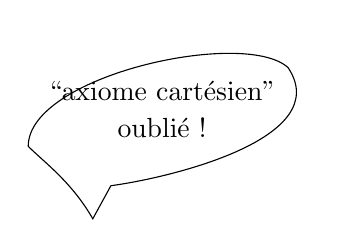
\begin{tikzpicture}
\node at (1.7,.85) {``axiome cartésien''};
\node at (1.7,.38) {oublié !};
\draw (0,.15) .. controls (0,1.05) and (2.75,1.65) .. (3.3,1.15)
.. controls (3.9,.25) and (1.8,-.25) .. (1.05,-.35)
--(.82,-.77) .. controls (.55,-.3) and (.2,-.05) .. (0,.15);
\end{tikzpicture}}}
\margin{
\diagram{
\begin{tikzcd}[column sep=small]
& X^{I\amalg I'\amalg I''} \arrow[dl,"p_{21}"'] \arrow[dr,"p_{32}"] &\\
X^{I\amalg I'} \arrow[dr,"\gamma'"'] && X^{I'\amalg I''} \arrow[dl,"\alpha'"] \arrow[dr,no head,"\alpha''"] &\\
& X^{I'} && X^{I''}
\end{tikzcd}
}
}
\[
\begin{aligned}
&=\alpha''_*\bigl(\underbrace{v\,p_{32*}\bigl(p_{21}^*(u)\,p_1^*(x)\bigr)}
_{\Vert\ \text{formule de projection, }\uline{\text{mod signe}}}\bigr)=\\
&\deleted{=\unsure{\alpha}}\quad
\underbrace{\alpha''_*p_{32*}}_{\Vert}\bigl(p_{32}^*(v)\,p_{21}^*(u)\,p_1^*(x)\bigr)\\
&\hspace{4em}p_{3*}\bigl(p_{32}^*(v)\,p_{21}^*(u)\,p_1^*(x)\bigr)
\end{aligned}
\]
\margin{OK mod \uline{signes}, à \unsure{faire} \uline{attention}}
\margin{45}
